\section{Hybrid 8-bit Floating-Point and 4-bit Logarithmic Computation}
\tableofcontents[currentsection]
\begin{frame}{Spike-by-Spike Neural Network}
	\begin{columns}[c] % The [T] option aligns the tops of the columns
		
		% Left column for the first image
		\begin{column}<1->{0.5\textwidth}
			\begin{figure}
				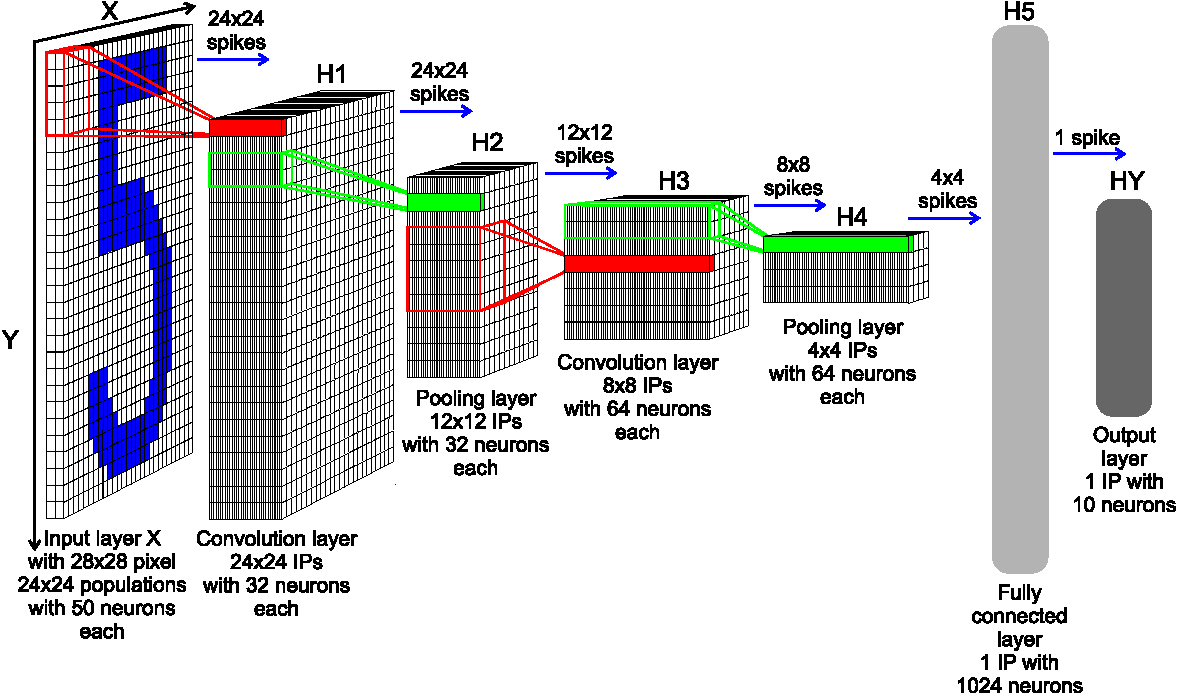
\includegraphics[width=\textwidth]{../chapters/sbs_accelerator/figures/sbs_network.pdf} % Adjust the filename
				\caption{Spike-by-Spike (SbS) neural network architecture for handwritten digit classification task}
			\end{figure}
		\end{column}
		
		% Right column for the second image
		\begin{column}<2->{0.5\textwidth}
			\begin{figure}
				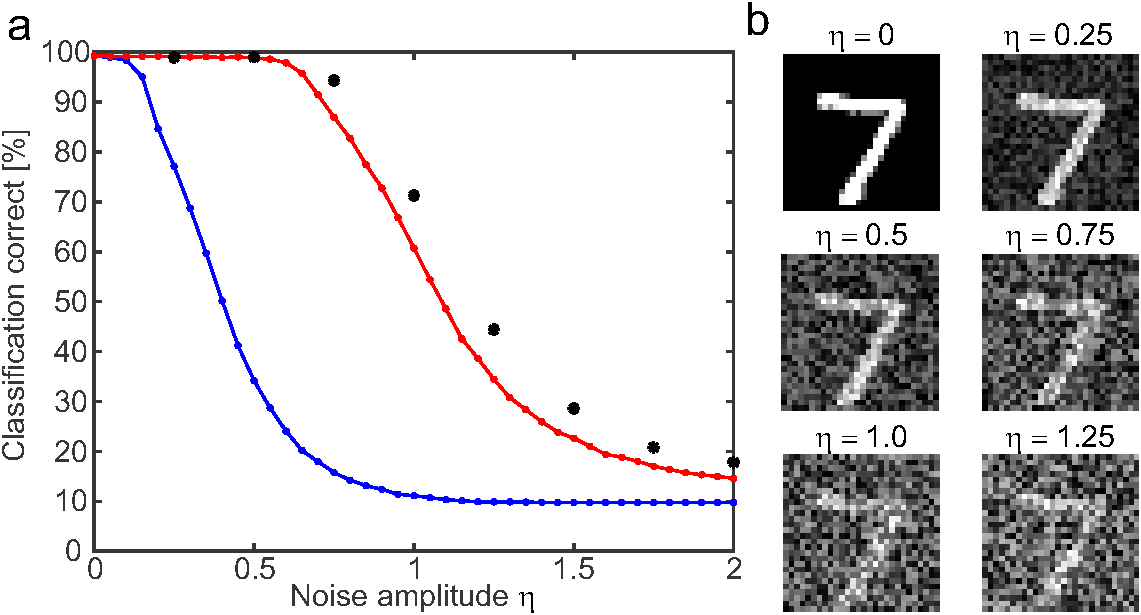
\includegraphics[width=\textwidth]{../chapters/sbs_accelerator/figures/sbs_robustnes.pdf} % Adjust the filename
				\caption{Performance classification of SbS NN versus equivalent CNN}
			\end{figure}
		\end{column}
		
	\end{columns}
\end{frame}

\begin{frame}{Spike-by-Spike Inference}
	\begin{figure}
		\centering
		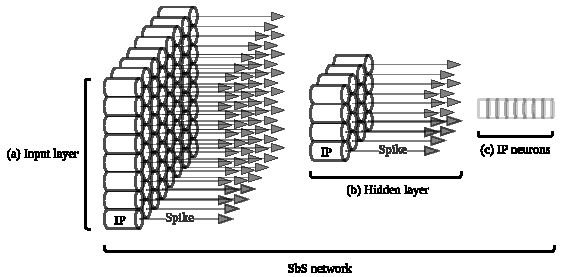
\includegraphics[width=0.5\textwidth]{../chapters/sbs_accelerator/figures/SbS_layer.pdf}
		\caption{SbS inference population (IP) as independent computational entities}
	\end{figure}
	
	%\pause % Pause for the equation to appear after the image
	
	% Equation at the bottom
	{
		\[
		h_\mu^{new}(i) = \frac{1}{1+\epsilon} \left(h_\mu(i) + \epsilon \frac{h_\mu(i) W(s_t|i) }{\sum_j h_\mu(j) W(s_t|j)} \right) 
		\]
	}
\end{frame}

\begin{frame}{HW/SW Co-Design and Deployment Framework}
	\begin{columns}[t] % The [T] option aligns the tops of the columns
		
		% Left column for the first image
		\begin{column}{0.5\textwidth}
			\begin{figure}
				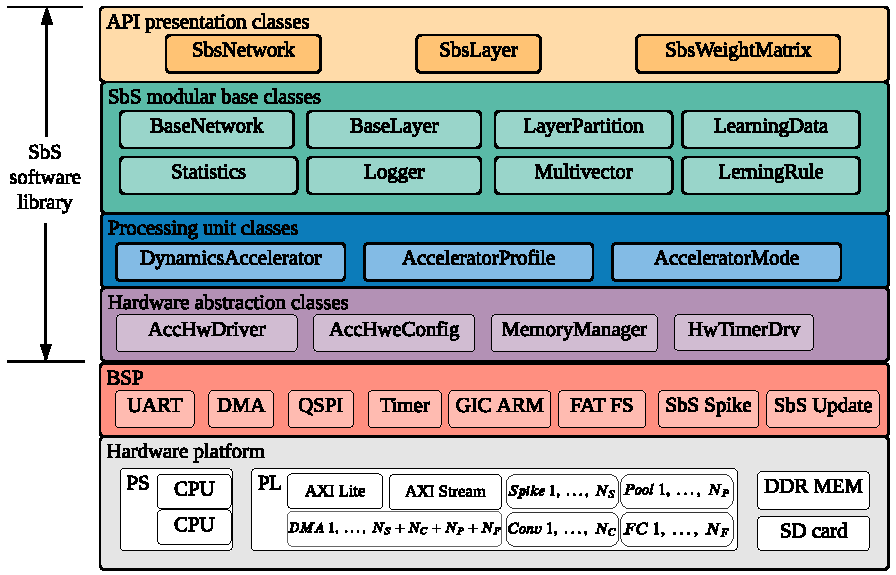
\includegraphics[width=0.8\textwidth]{../chapters/sbs_accelerator/figures/sbs_software_component.pdf}
				\caption{System-level overview of the embedded software architecture}
			\end{figure}
		\end{column}
		
		% Right column for the second image
		\begin{column}{0.5\textwidth}
			\begin{figure}
				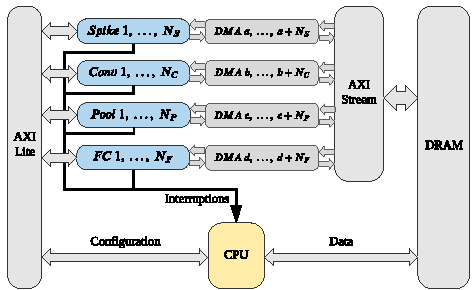
\includegraphics[width=0.8\textwidth]{../chapters/sbs_accelerator/figures/sbs_hw.pdf} % Adjust the filename
				\caption{System-level hardware architecture with scalable number of heterogeneous processing units}
			\end{figure}
		\end{column}
		
	\end{columns}
\end{frame}

\begin{frame}{Processing Unit}
	\begin{columns}[c] % The [T] option aligns the tops of the columns
		
		% Left column for the first image
		\begin{column}<1->{0.5\textwidth}
			\begin{figure}
				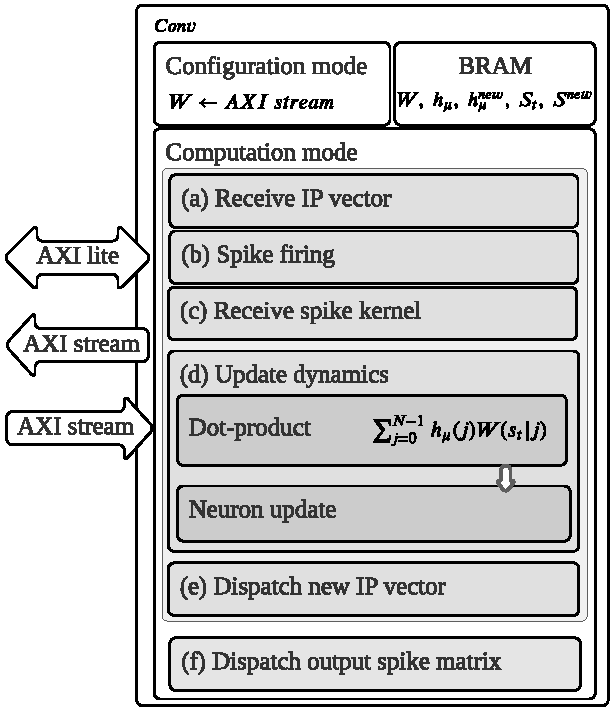
\includegraphics[width=0.7\textwidth]{../chapters/sbs_accelerator/figures/sbs_conv.pdf} % Adjust the filename
				\caption{Convolution processing unit}
			\end{figure}
		\end{column}
		
		% Right column for the second image
		\begin{column}<2->{0.5\textwidth}
			\begin{figure}
				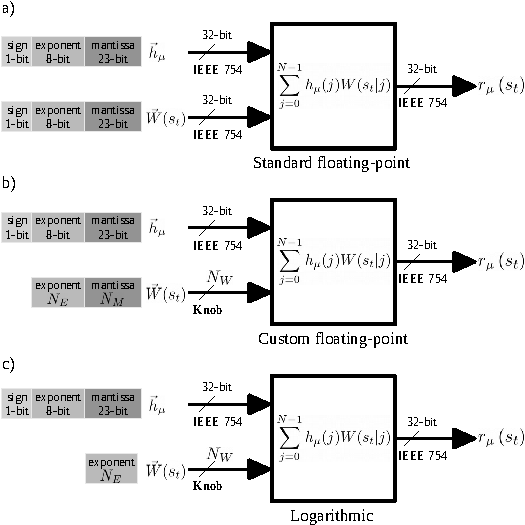
\includegraphics[width=0.9\textwidth]{../chapters/sbs_accelerator/figures/dot-product_unit.pdf} % Adjust the filename
				\caption{Dot-product hardware module}
			\end{figure}
		\end{column}
		
	\end{columns}
\end{frame}

\begin{frame}{Hybrid Dot-Product Approximation}
	\begin{columns}[c] % The [T] option aligns the tops of the columns
		% Left column for equations
		\begin{column}{0.5\textwidth}

			\begin{equation}
			r_{\mu}\left(s_t\right)=\sum_{j=0}^{N-1}h_{\mu}(j)W(s_t|j)
			\end{equation}
			\vspace{5mm} 
			\begin{equation}
			E_{\min}=\log _2(\min_{\forall i}(W(i)))
			\end{equation}
			\vspace{5mm} 
			\begin{equation}
			N_E=\lceil\log_2(|E_{\min}|)\rceil
			\end{equation}
			\vspace{5mm} 
			\begin{equation}
			N_W=N_E + N_M
			\end{equation}
		\end{column}
		
		% Right column for the image
		\begin{column}{0.5\textwidth}
			\begin{figure}
				\centering
				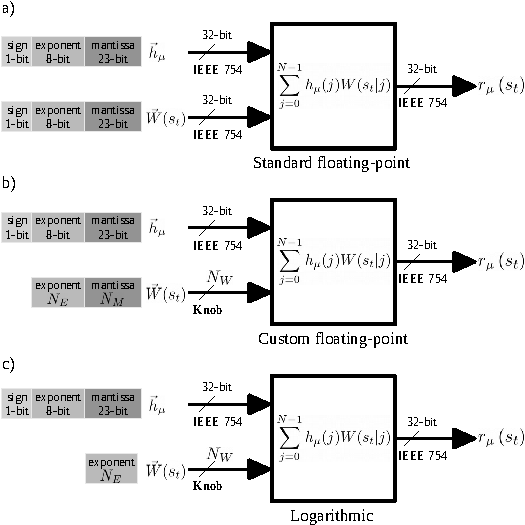
\includegraphics[width=0.9\textwidth]{../chapters/sbs_accelerator/figures/dot-product_unit.pdf} % Adjust the filename
				\caption{Dot-product hardware module}
			\end{figure}
		\end{column}
	\end{columns}
\end{frame}

\begin{frame}{Dot-Product with Standard Floating-Point (IEEE 754)}
	\begin{figure}
		\centering
		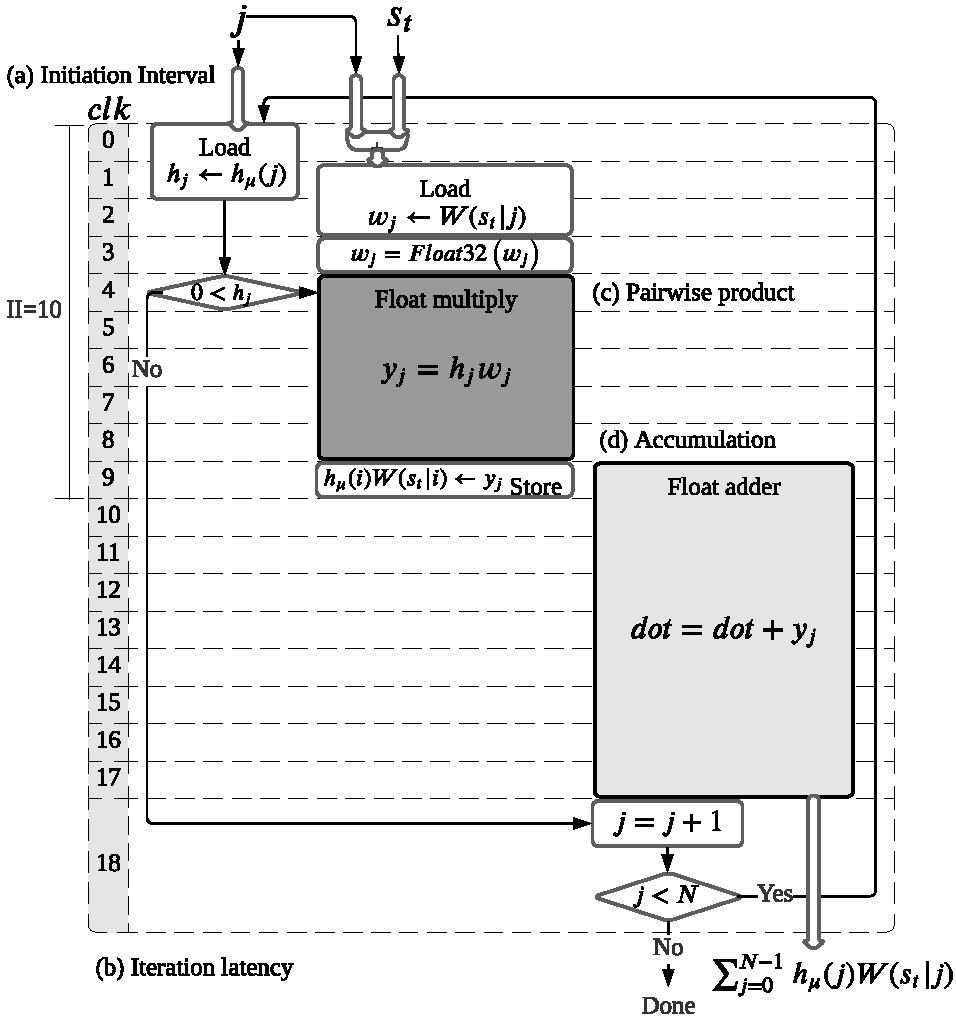
\includegraphics[width=0.4\columnwidth]{../chapters/sbs_accelerator/figures/dot_product_float.pdf}
		\caption{Dot-product hardware module with standard floating-point computation}
	\end{figure}
	
	\vfill % Add vertical space to push the equation to the bottom
	
	% Equation at the bottom
	\[
	 L_{f32}=10N+9
	\]
\end{frame}

\begin{frame}{Dot-Product with Hybrid Custom Floating-Point Approximation}
	\begin{figure}
		\centering
		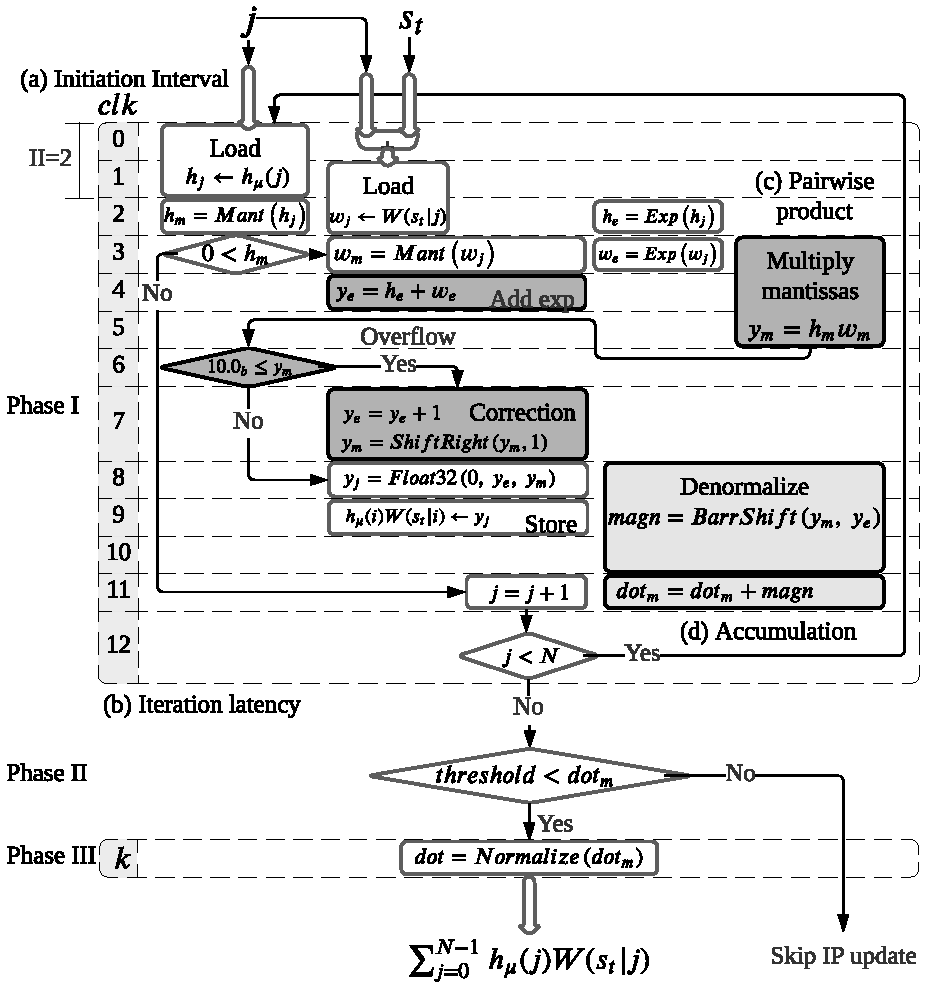
\includegraphics[width=0.4\columnwidth]{../chapters/sbs_accelerator/figures/dot_product.pdf}
		\caption{Dot-product hardware module with hybrid custom floating-point approximation}
	\end{figure}
	
	\vfill % Add vertical space to push the equation to the bottom
	
	% Equation at the bottom
	\[
	L_{custom}=2N+11
	\]
\end{frame}

\begin{frame}{Dot-product with Hybrid Logarithmic Approximation}
	\begin{figure}
		\centering
		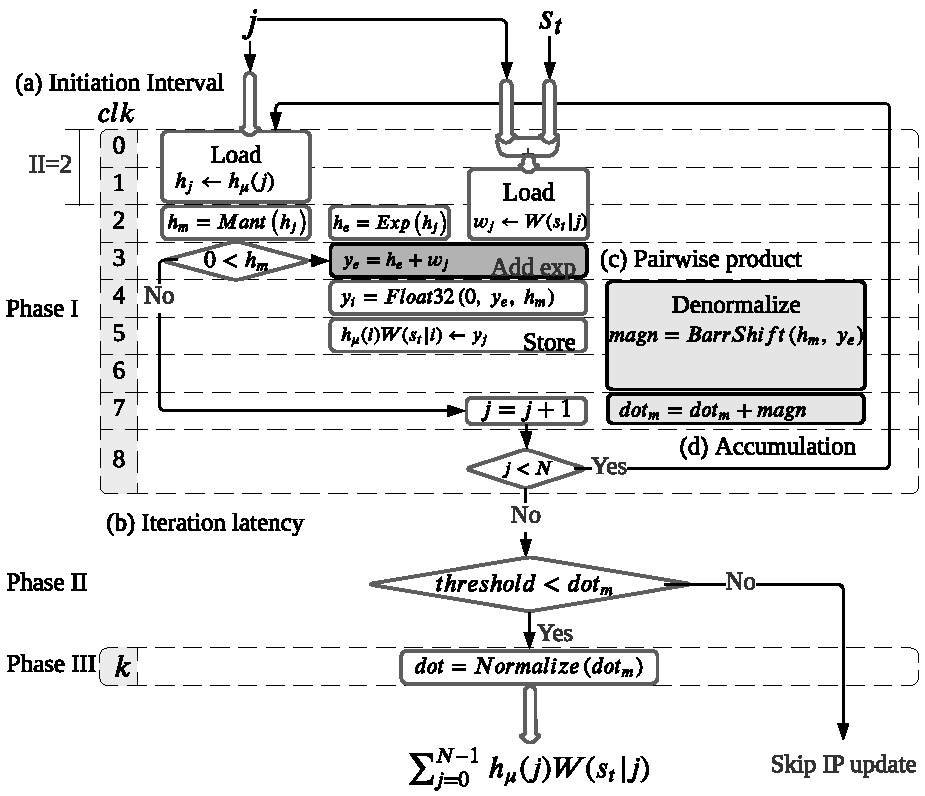
\includegraphics[width=0.4\columnwidth]{../chapters/sbs_accelerator/figures/dot_product_log.pdf}
		\caption{Dot-product hardware module with hybrid logarithmic approximation}
	\end{figure}
	
	\vfill % Add vertical space to push the equation to the bottom
	
	% Equation at the bottom
	\[
	L_{custom}=2N+7
	\]
\end{frame}

\begin{frame}{Deployment with Standard Floating-Point}
	\begin{columns}
		% Left Column
		\begin{column}{0.5\textwidth}
			% Top left image
			\begin{minipage}[c][.45\textheight][c]{\linewidth}
				\centering
				\begin{figure}
				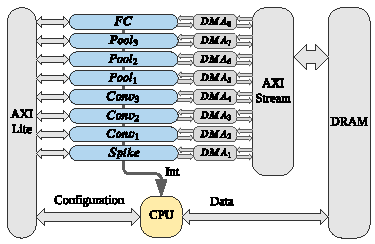
\includegraphics[width=0.75\linewidth]{../chapters/sbs_accelerator/figures/sbs_hw_experimental.pdf} % Adjust path and size as needed
				\caption{System overview of the top-level architecture with 8 processing units}
				\end{figure}
				\pause
			\end{minipage}
			
			% Bottom left image
			\begin{minipage}[c][.45\textheight][c]{\linewidth}
				\centering
				\begin{figure}
				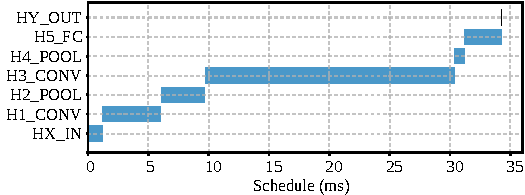
\includegraphics[width=0.75\linewidth]{../chapters/sbs_accelerator/figures/latency_sw.pdf} % Adjust path and size as needed
				\caption{Computation on embedded CPU}
				\end{figure}
				\pause
			\end{minipage}
		\end{column}
		
		% Right Column
		\begin{column}{0.5\textwidth}
			% Top right image
			\begin{minipage}[c][.45\textheight][c]{\linewidth}
				\centering
				\begin{figure}
				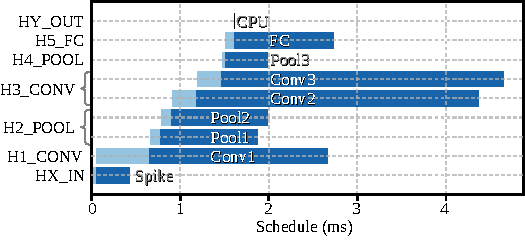
\includegraphics[width=0.75\linewidth]{../chapters/sbs_accelerator/figures/latency_pu_fp.pdf} % Adjust path and size as needed
				\caption{Performance of processing units with standard floating-point with \textbf{acceleration of 10.7X} }
				\end{figure}
				\pause
			\end{minipage}
			
			% Bottom right image
			\begin{minipage}[c][.45\textheight][c]{\linewidth}
				\centering
				\begin{figure}
				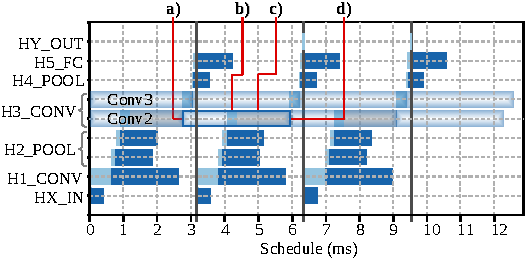
\includegraphics[width=0.75\linewidth]{../chapters/sbs_accelerator/figures/latency_fp_cycle.pdf} % Adjust path and size as needed
				\caption{Performance bottleneck of cyclic computation on processing units with standard floating-point}
				\end{figure}
			\end{minipage}
		\end{column}
	\end{columns}
\end{frame}

\begin{frame}{Deployment with Custom Floating-Point}
	\begin{columns}[c] % The [T] option aligns the tops of the columns
		
		% Left column for the first image
		\begin{column}<1->{0.5\textwidth}
			\begin{figure}
				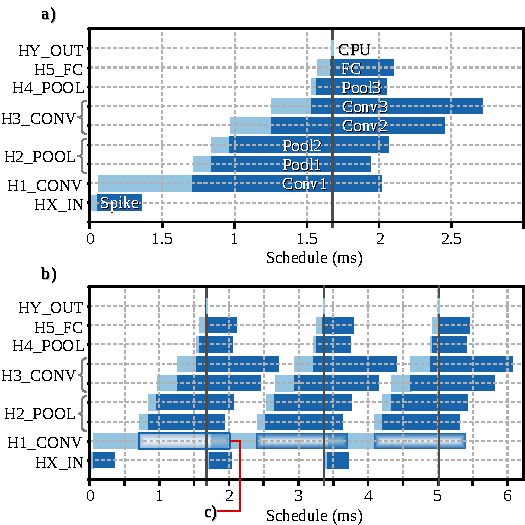
\includegraphics[width=0.75\textwidth]{../chapters/sbs_accelerator/figures/latency_cfp_cycle.pdf}
				 % Adjust the filename
				\caption{Performance on processing units with hybrid \textbf{8-bit floating-point} with \textbf{acceleration of 20.5X}}
			\end{figure}
		\end{column}
		
		% Right column for the second image
		\begin{column}<2->{0.5\textwidth}
			\begin{figure}
				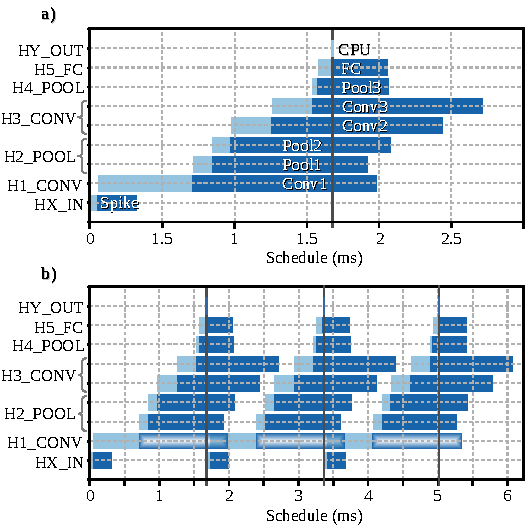
\includegraphics[width=0.75\textwidth]{../chapters/sbs_accelerator/figures/latency_log_cycle.pdf}
				\caption{Performance of processing units with hybrid \textbf{4-bit logarithmic} with \textbf{acceleration of 20.5X}}
			\end{figure}
		\end{column}
		
	\end{columns}
\end{frame}

\begin{frame}{Quantization Impact: Noise Tolerance}
	\begin{columns}
		% First column
		\begin{column}{0.33\textwidth}
			\centering
			\begin{figure}
			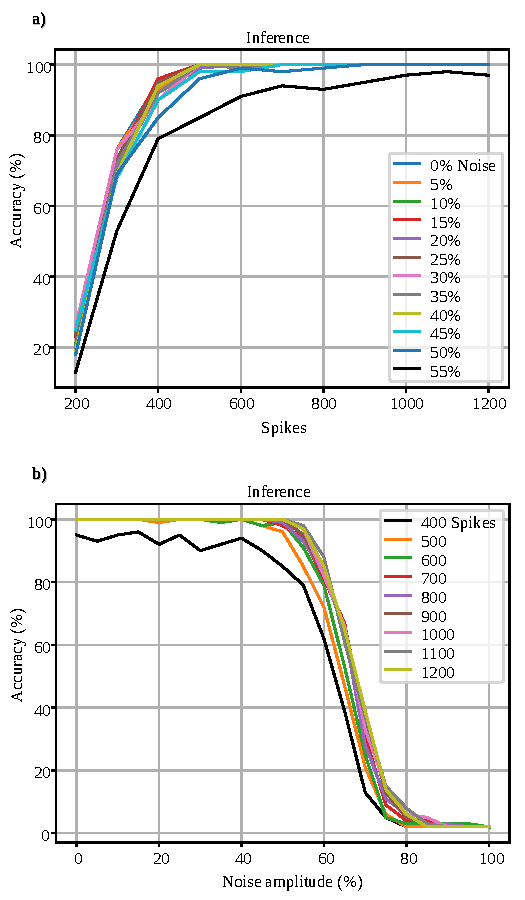
\includegraphics[width=0.75\linewidth]{../chapters/sbs_accelerator/figures/accuracy_vs_noise_pu_fp.pdf} % Adjust path and size as needed
			\caption{ Noise tolerance with \textbf{32-bit floating-point}}
			\end{figure}
			\pause
		\end{column}
		
		% Second column
		\begin{column}{0.33\textwidth}
			\centering
			\begin{figure}
			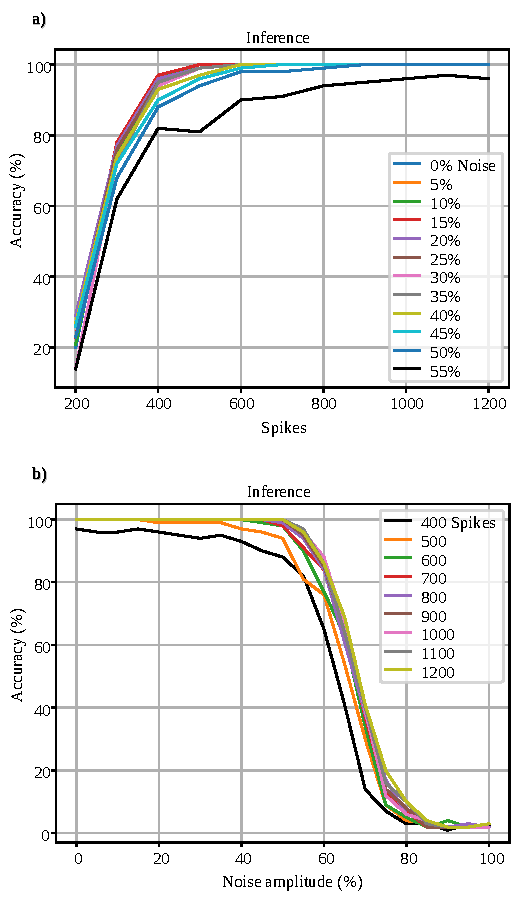
\includegraphics[width=0.75\linewidth]{../chapters/sbs_accelerator/figures/accuracy_vs_noise_pu_cfp(4-bit-exponent_1-bit-mantissa).pdf} % Adjust path and size as needed
			\caption{ Noise tolerance with hybrid \textbf{8-bit floating-point}}
			\end{figure}
			\pause
		\end{column}
		
		% Third column
		\begin{column}{0.33\textwidth}
			\centering
			\begin{figure}
			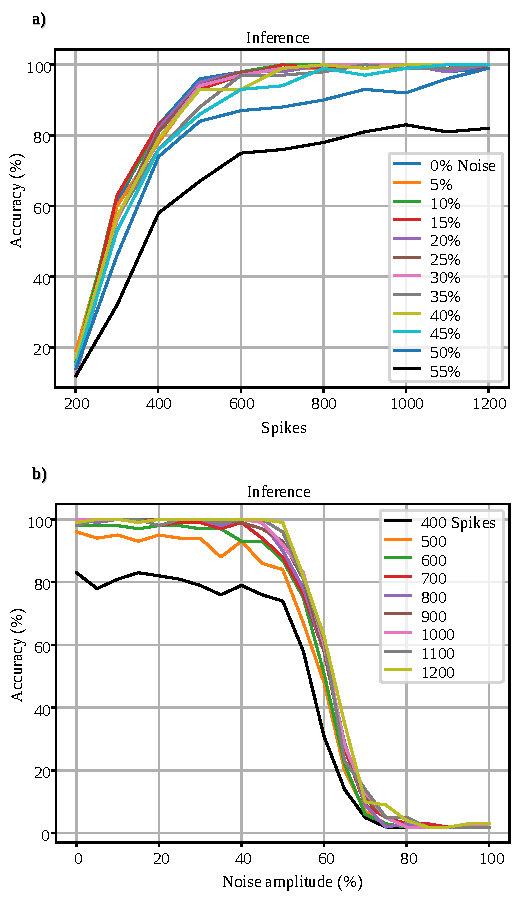
\includegraphics[width=0.75\linewidth]{../chapters/sbs_accelerator/figures/accuracy_vs_noise_pu_log.pdf} % Adjust path and size as needed
			\caption{ Noise tolerance with hybrid \textbf{4-bit logarithmic}}
			\end{figure}
		\end{column}
	\end{columns}
\end{frame}

\begin{comment}

\begin{frame}[shrink=30]{Accelerator Implementations} % Title of the slide
	\begin{center} % Ensure the table is centered in the slide
		\begin{threeparttable}
			\caption{Accelerator implementations.} % Caption of the table
			\scriptsize % Reduce the font size of the table
			\begin{tabular}{lrrrrr}
				\toprule
				\textbf{Platform implementation} & \textbf{Power (W)} & \textbf{Clk (MHz)} & \textbf{Latency (ms)} & \textbf{Acceleration} & \textbf{Accuracy (\%)} \\
				\midrule
				Standard floating-point & 2.420 & 200 & 3.18 & 10.7x & 98.98 \\
				Hybrid floating-point 8-bit & 2.369 & 200 & 1.67 & 20.5x & 98.97 \\
				Hybrid Logarithmic 4-bit & 2.324 & 200 & 1.67 & 20.5x & 98.84 \\
				\bottomrule
			\end{tabular}
		\end{threeparttable}
	\end{center}
\end{frame}

\end{comment}